\section{Background}

\subsection{Trajectory-planning}
A path for a robot can be described as a series of configurations that the robot should assume to go from a start to a goal configuration. The concept of configuration is described in \cite{ref:configurationSpace} as a set of independent parameters that describe the position of every point in a body.
\par
The terms path and trajectory are often used interchangeably. Formally, however, these terms are distinct. Path refers to, as mentioned before, all the consecutive configurations that a robot has to assume in order to go from a start to a goal configuration. In a trajectory, however, there has to be a timing law associated to the configurations that define the trajectory, for example having an associated speed and acceleration or time instant to each configuration in the trajectory \cite{ref:modelingPlanningControl}.

\subsection{IPOPT}
\label{subSeq:IPOPT}
In the present work, the used solver is an implementation of an interior point with a filter line-search method called IPOPT \cite{IPOPT}. The algorithm is complex and uses a primal-dual barrier method, originally developed by Andreas Wächter in \cite{ref:IPOPTthesis}, inspired in previous work by Fiacco et al. \cite{fiacco}.
\par
In sequential quadratic programming (SQP) there is the need to identify the active bound constraints. Barrier problems avoid this problem by replacing the constraints for logarithmic terms in the cost function. Thus being said, barrier methods solve optimization problems of the type:

\begin{equation}
    \begin{matrix}
    \text{min:} && \quad f(x) && \\
    \text{s.t.:} && \quad c(x)=0 && \\
     && \quad  x_i > 0 && , i \in \mathcal{I}
    \end{matrix}
    \label{eq:barrierProblem}
\end{equation}

where $\mathcal{I}$ defines the set of indexes of bounded variables.
By converting the problem into the following one, stated in Equation \ref{eq:barrierFormulation}, called a \textit{barrier problem}:

\begin{equation}
    \begin{matrix}
    \text{min:} && \quad \phi_\mu (x) = f(x) - \mu \sum_{i \in \mathcal{I}} ln(x_i) \\
    \text{s.t.:} && \quad c(x)=0
    \end{matrix}
    \label{eq:barrierFormulation}
\end{equation}

where $\mu$ is the barrier parameter, which is greater than 0. This formulation imposes that $ x_i > 0$ for $ i \in \mathcal{I}$ because, as $x_i$ tends to 0, the value of $\phi_\mu (x)$, the barrier function, tends to infinite. The formulation in Equation \ref{eq:barrierFormulation} matches the problem defined in Equation \ref{eq:barrierProblem} for $\mu \rightarrow 0$. For $\mu > 0$, it becomes clear that the solution never lies in the boundary of the problem, instead it always lies in the interior of the desired design variable region. For this reason, the barrier methods are also called interior point methods. In these methods, multiple sub-problems (barrier problems) are solved for decreasing values of $\mu$. 
\par
IPOPT allows solving general dual-barrier problems of the type:

\begin{equation}
    \begin{matrix}
    \text{min:} && \quad f(x) && \\
    \text{s.t.:} && \quad c(x) = 0 && \\
     && \quad  x_{i l} < x_i < x_{i u} && , i \in \mathcal{I} \\
     && \quad  d_{l} < d(x) < d_{u} && \\
    \end{matrix}
    \label{eq:IPOPTProblem}
\end{equation}

where $x_{i l}$ and $x_{i u}$ are lower and upper boundaries for $x_i$. $d_{l}$ and $d_j(x)$ are lower and upper boundaries for the inequality functions $d(x)$. In order to convert the typical barrier problem stated in \ref{eq:barrierProblem} into the more general form shown in \ref{eq:IPOPTProblem}, it is required to, instead of using the variables $v_i=\frac{\mu}{x}$, create  the variables $v_{i l}= \frac{\mu}{x_i-x_{i l}}$ and $v_{i u}= \frac{\mu}{x_{i u}-x_{i}}$. Doing this,  the equalities forcing these new definitions of $v_{ i l}$ and $v_{i u}$ become $v_{ i l} * (x-x_{i l})=\mu$ and $v_{ i u} * (x_{i u}-x_i)=\mu$ respectively.
\par
In order to explain how IPOPT deals with inequalities defined by general functions $d(x)$, it is defined an isolated inequality:

\begin{equation}
  d_{j l} < d_j(x) < d_{j u}
\end{equation}

where $d_j(x)$ represents the $j$th inequality function and $d_{j l}$ and $d_{j u}$ represent the respective lower and upper bounds. These inequalities are changed to a set of equalities and inequalities shown in Equation \ref{newInequalities} by introducing slack variables $s_j$:

\begin{equation}
    \begin{matrix}
       d_j(x)-s_j=0\\
       d_{j l} < s_j < d_{j u}
    \end{matrix}
    \label{newInequalities}
\end{equation}

The equalities are treated then as regular equalities. The inequalities $d_{j l} < s_j < d_{j u}$ are then imposed in the same way as the inequalities $x_{i l} < x_i < x_{i u}$.

\subsection{Trajectory Optimization}
Optimization techniques can be used to compute trajectories. However,  it is required to state an optimization problem in such a way that its solution can be used to compute a trajectory. In \cite{ref:optimizationReview}, an overview of trajectory optimization techniques and applications is performed. Besides giving an overview in numerical methods for optimization, in \cite{ref:optimizationReview} a series of traditional formulations of trajectory planning problems as optimization problems is given. Usually, in these problems, the system dynamics is imposed using equality constraints such as:

\begin{equation}
    \dot{\sigma} = f(\sigma, u)
\end{equation}

where $\sigma$ represents the system state and $u$ the control inputs. Nevertheless,  these equalities must be formulated in a discrete-time domain. To achieve this, the derivatives $\dot{\sigma}$ are usually taken using finite differentiation.
\par
Trajectory optimization has been applied also to multi-rotors. In \cite{ref:quad}, optimization is only used to compute splines joining way-points in a previously computed trajectory. On other works, such as \cite{MILP, ETH}, trajectory optimization is used to completely compute trajectories from naive first iterations. The approach taken to describe the trajectory varies. In \cite{MILP}, the trajectories are discretized into a series of way-points, unlike in \cite{ETH} where trajectories are described as a series of high order splines, which parameters are optimized.
\par
To sum up, in order to perform trajectory optimization it is required to choose a finite set of parameters to describe the trajectory, such as a set of way-points or a sequence of control inputs, and then formulate the problem in such a way that the system dynamic and actuation limits of the problem are respected. Finally, a cost function must be chosen to minimize.

\subsection{Multi-rotor-rotor dynamics}
 It is now introduced the concepts of inertial frame and body frame. The inertial frame is, as the name suggests, a frame that moves in a constant speed (or static), where the $z_w$ axis is aligned with the vertical, pointing upwards. The body frame is fixed to the multi-rotor and the $z_b$ is perpendicular to the rotor plane and points up when the multi-rotor is hovering. A representation of these frames is shown in Fig \ref{fig:framesUAV}.
 \par
As stated in \cite{ref:mellingerFlat}, the UAV state can be written as the position of its center of mass ($x$, $y$ and $z$), the speed of the center of mass ($\dot{x}$, $\dot{y}$ and $\dot{z}$), the roll pitch and yaw angles ($\phi$,$\theta$ and $\psi$) and the angular velocities around the body axis $x_b$, $y_b$ and $z_b$ ($p$, $q$ and $r$ respectively).
\par

 
 \begin{equation}
     \sigma=[x,y,z,\phi, \theta, \psi, \dot{x}, \dot{y}, \dot{z}, p, q, r]^T
 \end{equation}
 
 The inputs are considered to be the resulting force along the $z_b$ component of the body frame of the vehicle ($u_4$) and the moments along $x_b$, $y_b$ and $z_b$ of the vehicle ($u_1$, $u_2$ and $u_3$). This thrust and moments are assumed to be given linearly from the square of each rotor speed ($\omega_1^2$, ... , $\omega_4^2$). It is also assumed that the rotor speeds can be directly controlled. Let $u=[u_1, u_2, u_3, u_4]^T$ and $\omega^2 = [\omega_1^2$, ... , $\omega_4^2]^T$. For multi-rotors with more rotors, the control input $u$ will be the same (thrust along the axis perpendicular to the rotors plane $z_b$ and moments applied to the center of mass), once a series of rotors that provide thrust in the same direction are only capable of generating force along that same direction. To map from the squared rotation speed of $n$ rotors $\omega^2$ into control inputs $u$, as described before, it is used a matrix usually called allocation matrix $A$ $4 \times n$, such as in Equation \ref{eq:allocMatrix}.
 
 \begin{equation}
     u=A [\omega_1^2, ... , \omega_n^2]^T
     \label{eq:allocMatrix}
 \end{equation}
 
 It is clear that for more than 4 rotors the matrix does not have an inverse. For that reason, when it is desired to map $u$ into $[\omega_1^2, ... , \omega_n^2]$, with $n>4$, it is necessary to add some extra constraints to the system.
 
 \begin{figure}[ht!]
     \centering
     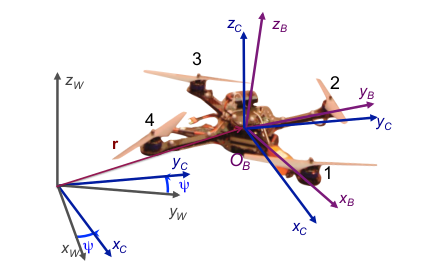
\includegraphics[width=0.8\linewidth]{Figures/02_background/frames.png}
     \caption{Inertial frame (subscript W) and body frame (subscript B) of a multi-rotor. Taken directly from \cite{ref:mellingerFlat}}
     \label{fig:framesUAV}
 \end{figure}

\subsection{Quad-rotor differential flatness}
 
  In \cite{ref:mellingerFlat}, it is proven that a quad-rotor is a differentially flat system. This implies that it is possible to compute the control inputs and the UAV configuration from a trajectory defined in the flat output space \cite{ref:diffFlat}.
 
 The flat outputs chosen in this work were the vehicles center of mass coordinates in the inertial frame ($x_w$, $y_w$ and $z_w$) and the yaw angle ($\psi$). The trajectories will be computed for the center of mass position in the inertial frame and the yaw angle ($\psi$) will be considered as constant and equal to 0, there is however the freedom to control the yaw angle which might be useful for, for example, directing a camera fixed to the UAV.
 
 \begin{equation}
     w = \left [ x, y, z, \psi \right ]^T
 \end{equation}
 
 The authors provide expressions for computing the quad-rotor state $\sigma$ and inputs $u$ from the flat output variables and their derivatives up to the fourth derivative. This means that it is possible for the quad-rotor to follow the computed trajectory in the flat output space (position and yaw) as long as the inputs are not saturated.

 \subsection{Approximated dynamics}
 In this work, like in some others \cite{ref:quad, MILP}, a first approximation is made, considering that the acceleration of the vehicle can be directly controlled (ignoring attitude information). In such approximated system, the UAV can be described as a point with a mass, and its state considers only the position of the center of mass and the speed.  This approximation, however, leads to generated trajectories that can not be followed by the real quad-rotor. Discontinuities on the acceleration direction would translate into discontinuities in the vehicle attitude (the $z_b$ axis of the body frame must be aligned with the acceleration vector at all times). If it is desired to make use of the differential flatness propriety, computing directly the control inputs from the flat output variables (from a trajectory in 3-dimensional space with freedom to control the yaw angle), it is required to have information on the flat output variables up to the $4^{th}$ derivative (snap and $4^{th}$  derivative of yaw angle with respect to time). This can be achieved by smoothing the trajectory, as it is made in \cite{ref:quad}.
 \par
 In the present work, the computed trajectories only provide information up to the $2^{nd}$ derivative of the position. It is then desirable to have a suitable controller for the case, once the inputs can not be directly taken from the computed trajectory. The chosen controller is based on the work by Lee et al. \cite{Lee}. Further on this work, this approximation is validated using experimental data.
 